\documentclass{article}


% if you need to pass options to natbib, use, e.g.:
%     \PassOptionsToPackage{numbers, compress}{natbib}
% before loading neurips_2023


% ready for submission
% \usepackage{neurips_2023}


% to compile a preprint version, e.g., for submission to arXiv, add add the
% [preprint] option:
  \usepackage[preprint]{neurips_2023}


% to compile a camera-ready version, add the [final] option, e.g.:
  % \usepackage[final]{neurips_2023}


% to avoid loading the natbib package, add option nonatbib:
  %  \usepackage[nonatbib]{neurips_2023}


\usepackage[utf8]{inputenc} % allow utf-8 input
\usepackage[T1]{fontenc}    % use 8-bit T1 fonts
\usepackage{hyperref}       % hyperlinks
\usepackage{url}            % simple URL typesetting
\usepackage{booktabs}       % professional-quality tables
\usepackage{amsfonts}       % blackboard math symbols
\usepackage{nicefrac}       % compact symbols for 1/2, etc.
\usepackage{microtype}      % microtypography
\usepackage{xcolor}         % colors
\usepackage{graphicx}       % Required for including graphics
\usepackage{subcaption}     % Required for subfigure environment
\usepackage{listings}       % Required for lstlisting environment
\usepackage{float}          % Enables tables to be rendered anywhere on the page
\usepackage{amsmath}        % For math environments like equation
\usepackage{pgfplots}       % For histogram
\usepackage{tikz}           % For histogram
\pgfplotsset{compat=1.18}


\title{BME1312 Project2 Report: Deep Learning Cardiac Cine MRI Segmentation}


% The \author macro works with any number of authors. There are two commands
% used to separate the names and addresses of multiple authors: \And and \AND.
%
% Using \And between authors leaves it to LaTeX to determine where to break the
% lines. Using \AND forces a line break at that point. So, if LaTeX puts 3 of 4
% authors names on the first line, and the last on the second line, try using
% \AND instead of \And before the third author name.


\author{%
  Wenye Xiong \\
  2023533141 \\
  \texttt{xiongwy2023@shanghaitech.edu.cn}
  \And
  Renyi Yang \\
  2023533030 \\
  \texttt{yangry2023@shanghaitech.edu.cn}
  \AND
  Jiaxing Wu \\
  2023533160 \\
  \texttt{wujx2023@shanghaitech.edu.cn}
  \And
  Boyang Xia \\
  2023533073 \\
  \texttt{xiaby2023@shanghaitech.edu.cn}
  \AND
  Fengmin Yang \\
  2023533183 \\
  \texttt{yangfm2023@shanghaitech.edu.cn}
}

\begin{document}


\maketitle


\begin{abstract}
  This report details the implementation and evaluation of U-Net based deep learning models for cardiac segmentation
  in cine MRI scans. The project focuses on segmenting three key structures: the Left Ventricle (LV), Right Ventricle (RV),
  and Myocardium (MYO). We explore the standard U-Net architecture, the impact of removing skip connections, the effect of
  data augmentation, the performance difference between Binary Cross-Entropy loss and Soft Dice loss, and potential improvements using an Attention U-Net and Hybrid Loss.
\end{abstract}

\section{Introduction}
The primary goal of this project is to segment key cardiac structures, namely the Left Ventricle (LV), Myocardium (MYO), and Right Ventricle (RV), from cine MRI scans. A significant challenge lies in the accurate and robust delineation of these structures, which can exhibit considerable variability in shape and appearance across different patients and image acquisitions.

To address this, we employ a U-Net based deep learning framework. Our approach involves several stages:
\begin{itemize}
  \item Implementing a baseline U-Net model.
  \item Investigating the impact of removing U-Net skip connections.
  \item Evaluating the effect of data augmentation techniques.
  \item Comparing the performance of Binary Cross-Entropy (BCE) loss versus Soft Dice Loss.
  \item Exploring improvements to the U-Net architecture by incorporating attention mechanisms (Attention U-Net) and a Hybrid Loss function.
\end{itemize}
The performance of all models is primarily evaluated using the Dice Similarity Coefficient (DSC).

\section{Baseline U-Net}

\subsection{Structure}
The U-Net architecture, as depicted in Figure \ref{fig:network_architecture}, consists of:
\begin{itemize}
  \item \texttt{DoubleConv}: A block of two sequential (Conv2D 3x3, BatchNorm2D, ReLU) operations.
  \item \texttt{Down}: Max pooling (2x2) followed by a \texttt{DoubleConv} block for downsampling in the encoder.
  \item \texttt{Up}: Upsampling (bilinear or transpose convolution) followed by concatenation with features from the
        corresponding encoder layer (skip connection) and a \texttt{DoubleConv} block. Padding is used to handle potential
        size mismatches during concatenation.
\end{itemize}

Our baseline is as below:
\begin{itemize}
  \item \textbf{Network}: The standard \texttt{UNet} class as described above, with \texttt{C\_base=32}, 1 input channel,
        and 3 output classes. Bilinear upsampling was used.
  \item \textbf{Loss Function}: A custom \texttt{MyBinaryCrossEntropy} loss was used. This involves applying a Sigmoid
        function to the model's output logits to get probabilities, then computing \texttt{nn.BCELoss} against the 3-channel
        binary ground truth masks. The learning rate was 0.01, and training was run for 50 epochs.
  \item \textbf{Evaluation}: Mean and standard deviation of the Dice Similarity Coefficient (DSC) for LV, RV, and MYO
        were calculated on the test set. Training and validation loss curves were plotted.
        Example segmentation results were saved.
\end{itemize}

\begin{figure}[H]
  \centering
  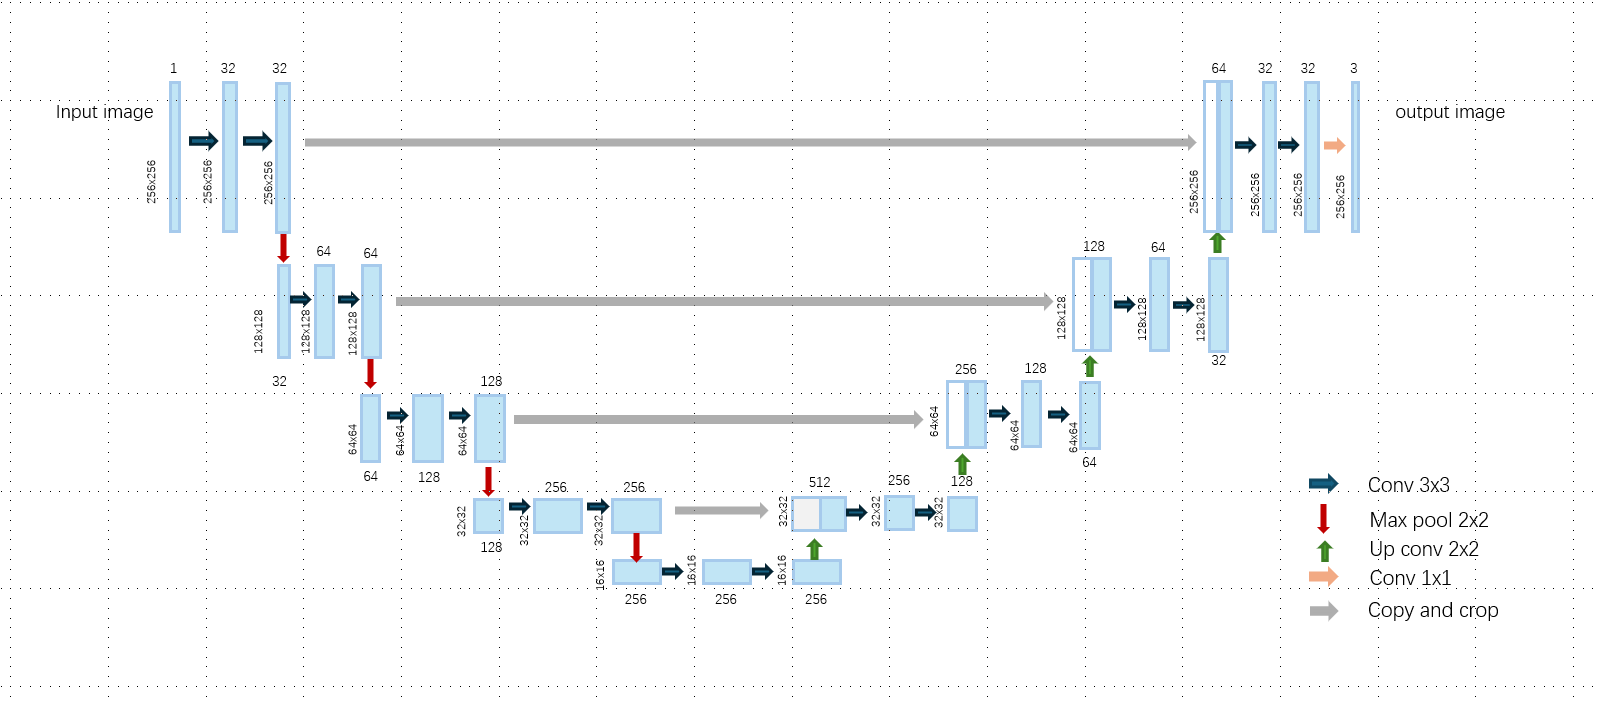
\includegraphics[width=1\linewidth]{../result/network.png}
  \caption{U-Net Network Architecture.}
  \label{fig:network_architecture}
\end{figure}

\subsection{Experiments and Results}
The training loss and validation loss of the baseline U-Net are shown in Figure \ref{fig:baseline_unet_loss}.
\begin{figure}[H]
  \centering
  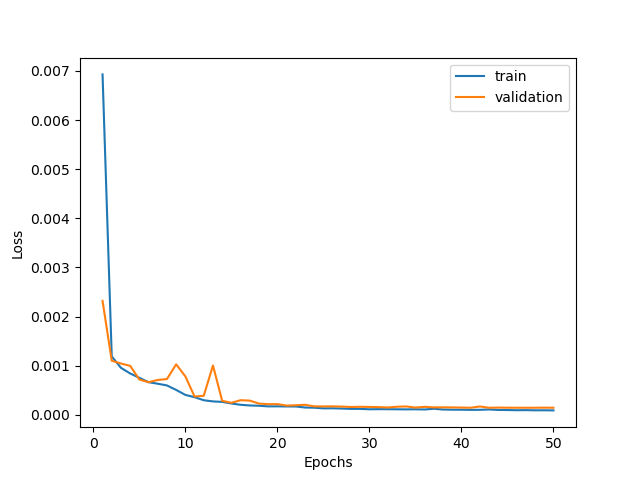
\includegraphics[width=\linewidth]{../result/baseline_unet.png}
  \caption{Training and Validation Loss Curves for the Baseline U-Net}
  \label{fig:baseline_unet_loss}
\end{figure}

And here are example segmentation results in Figure \ref{fig:baseline_unet_segmentation_example_lv},
\ref{fig:baseline_unet_segmentation_example_myo}, and \ref{fig:baseline_unet_segmentation_example_rv}.
\begin{figure}[H]
  \centering
  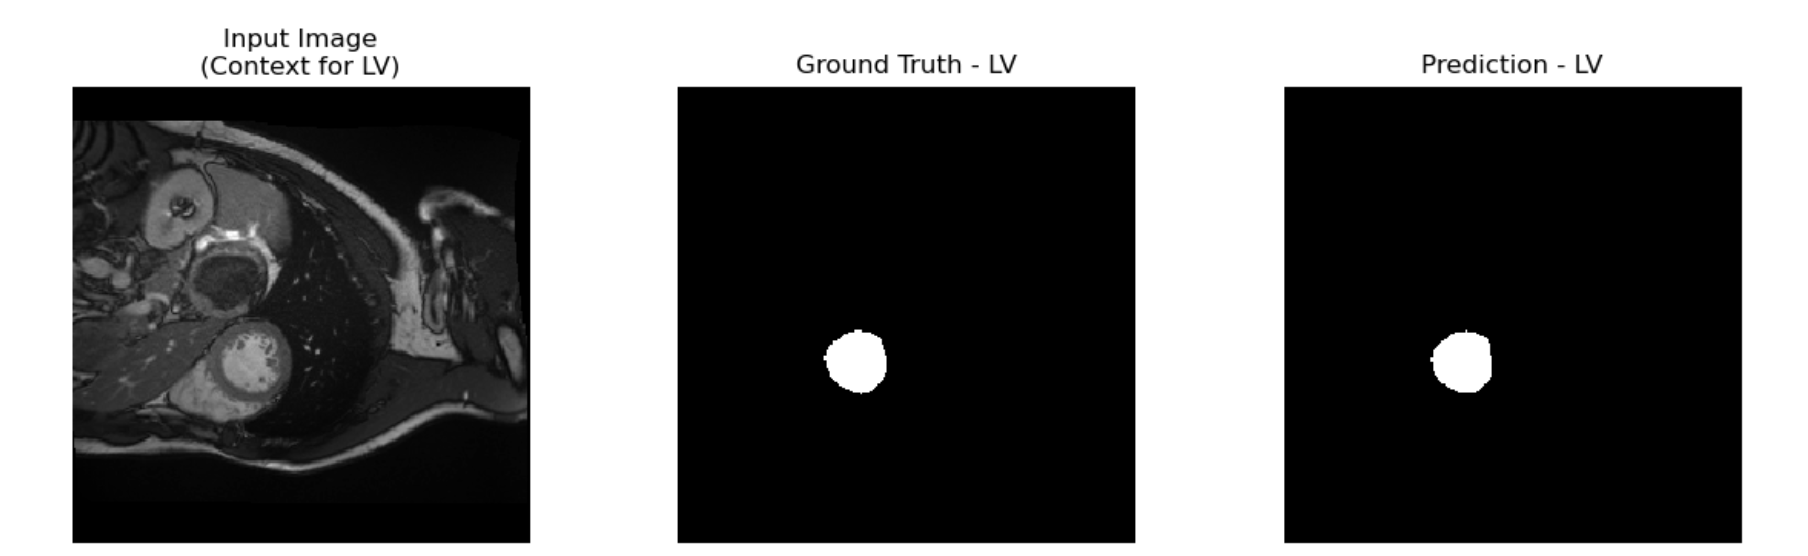
\includegraphics[width=\linewidth]{../result/for_ppt/baseline_LV.png}
  \caption{Baseline U-Net Segmentation Example: LV}
  \label{fig:baseline_unet_segmentation_example_lv}
\end{figure}
\begin{figure}[H]
  \centering
  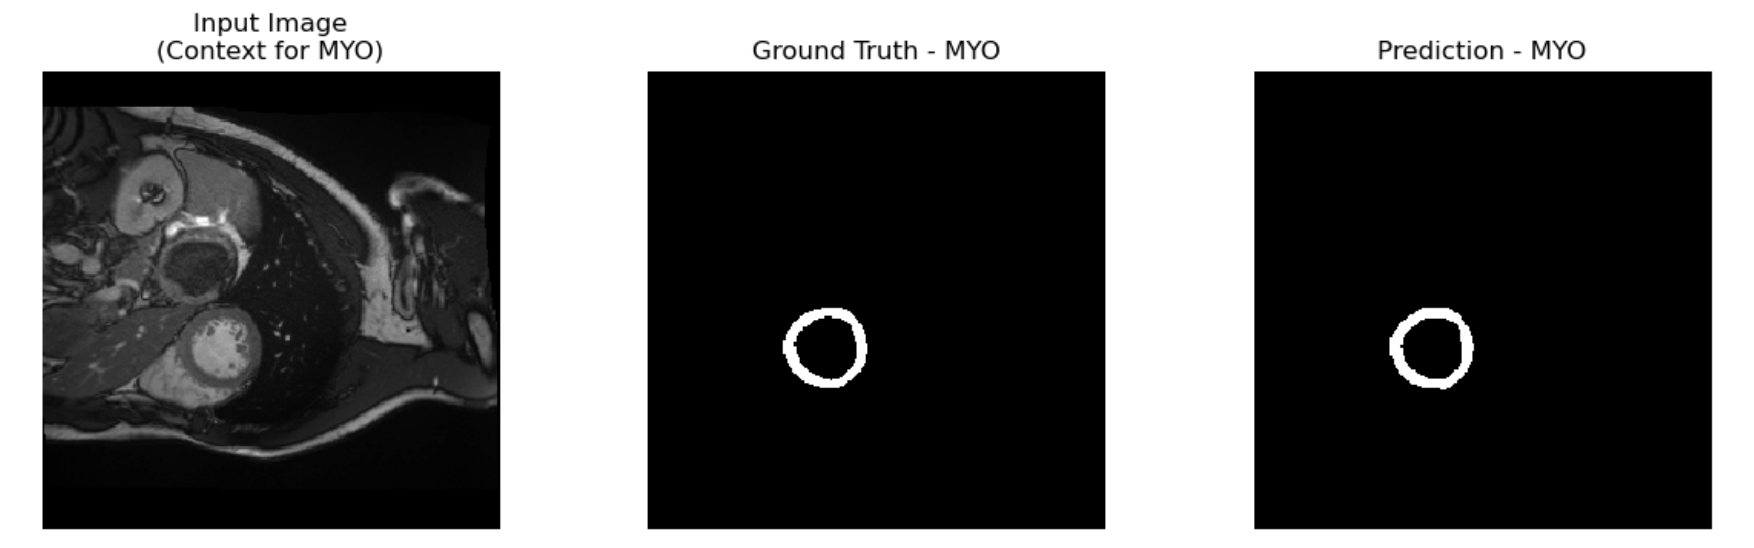
\includegraphics[width=\linewidth]{../result/for_ppt/baseline_MYO.png}
  \caption{Baseline U-Net Segmentation Example: MYO}
  \label{fig:baseline_unet_segmentation_example_myo}
\end{figure}
\begin{figure}[H]
  \centering
  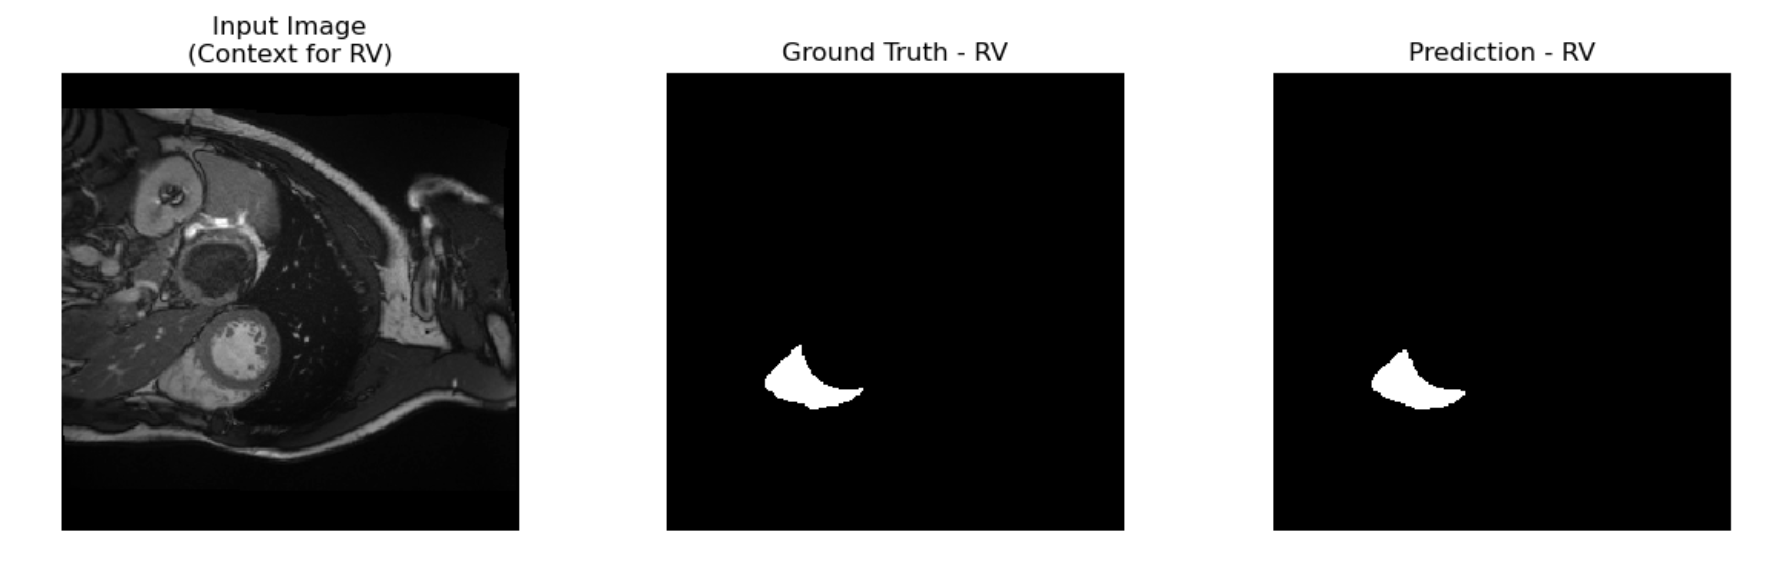
\includegraphics[width=\linewidth]{../result/for_ppt/baseline_RV.png}
  \caption{Baseline U-Net Segmentation Example: RV}
  \label{fig:baseline_unet_segmentation_example_rv}
\end{figure}

The baseline U-Net trained with Cross-Entropy loss achieved the following Dice scores (Table \ref{tab:baseline_unet}):
\begin{table}[H]
  \centering
  \caption{Dice Coefficients for Baseline U-Net (Task a)}
  \label{tab:baseline_unet}
  \begin{tabular}{lcc}
    \toprule
    Structure & Mean Dice & Standard Deviation \\
    \midrule
    RV        & 0.9519    & 0.0086             \\
    MYO       & 0.8734    & 0.0161             \\
    LV        & 0.8920    & 0.0310             \\
    \bottomrule
  \end{tabular}
\end{table}

\subsection{Discussion}
The baseline U-Net (Table \ref{tab:baseline_unet}) demonstrated strong segmentation performance.
\begin{itemize}
  \item \textbf{RV Segmentation}: Achieved the highest mean Dice score (0.9519). This is often expected as the RV is typically a large, relatively well-defined structure with good contrast against surrounding tissues in many MRI sequences.
  \item \textbf{LV Segmentation}: Also showed good performance with a mean Dice of 0.8920. The LV cavity is usually clearly visible.
  \item \textbf{MYO Segmentation}: Had the lowest mean Dice score (0.8734). The myocardium is a thinner, more complex structure surrounding the LV, and its boundaries, especially with the LV cavity (endocardium) and epicardium, can be more challenging to delineate accurately, potentially leading to lower overlap scores.
  \item The standard deviations are relatively small, indicating consistent performance across the test slices. Overall, the baseline U-Net provides a solid foundation for cardiac segmentation.
\end{itemize}


\section{U-Net without Skip Connections}

\subsection{Structure}
\begin{itemize}
  \item \textbf{Network Modification}: A \texttt{UNet\_NoShortcut} model was implemented. This involved creating an
        \texttt{Up\_NoShortcut} module that performs upsampling and convolution but does not concatenate features from the encoder
        path. The \texttt{forward} method of \texttt{Up\_NoShortcut} only processes the feature map from the previous decoder layer.
  \item \textbf{Retraining}: This modified U-Net was trained following the same procedure as the baseline U-Net: 50 epochs, Adam optimizer, learning rate of 0.01, and \texttt{MyBinaryCrossEntropy} loss.
  \item \textbf{Purpose}: Evaluate the importance of skip connections.
\end{itemize}

\subsection{Performance}
The training and validation loss curves for the U-Net without skip connections are shown in Figure \ref{fig:no_shortcut_loss}.
\begin{figure}[H]
  \centering
  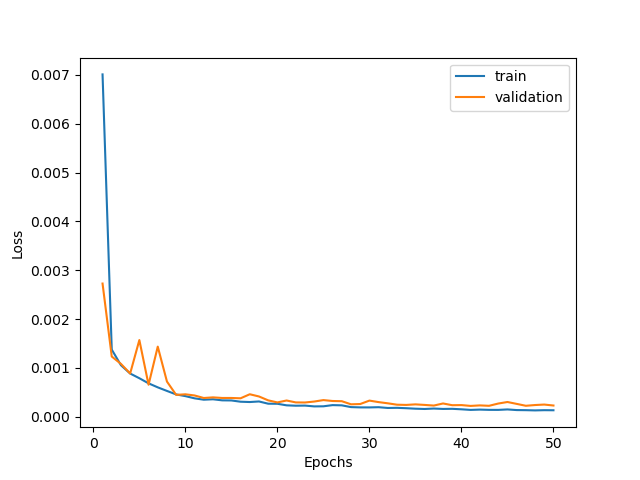
\includegraphics[width=0.8\linewidth]{../result/no_shortcut_unet.png}
  \caption{Training and Validation Loss for U-Net without Skip Connections.}
  \label{fig:no_shortcut_loss}
\end{figure}

The U-Net variant without skip connections, trained under identical conditions, yielded the Dice coefficients shown in Table \ref{tab:no_shortcut_unet_comparison}.
\begin{table}[H]
  \centering
  \caption{Dice Coefficients: Baseline U-Net vs. U-Net without Skip Connections (Task b)}
  \label{tab:no_shortcut_unet_comparison}
  \begin{tabular}{l|cc|cc}
    \toprule
    Structure & \multicolumn{2}{c|}{Baseline U-Net (DSC)} & \multicolumn{2}{c}{U-Net No Shortcut (DSC)}                         \\
              & Mean Dice                                 & Std. Dev.                                   & Mean Dice & Std. Dev. \\
    \midrule
    RV        & 0.9519                                    & 0.0086                                      & 0.9260    & 0.0111    \\
    MYO       & 0.8734                                    & 0.0161                                      & 0.8223    & 0.0168    \\
    LV        & 0.8920                                    & 0.0310                                      & 0.8588    & 0.0296    \\
    \bottomrule
  \end{tabular}
\end{table}

\subsection{Discussion}
Comparing the performance in Table \ref{tab:no_shortcut_unet_comparison}, removing skip connections resulted in a significant drop in performance across all structures.
\begin{itemize}
  \item \textbf{Significant Drop in Performance}: All structures showed a noticeable decrease in DSC.
  \item \textbf{Reason}: Skip connections provide high-resolution spatial information from the encoder to the decoder, which is crucial for accurate boundary localization. They also aid gradient flow during backpropagation, mitigating vanishing gradient problems and improving convergence.
  \item \textbf{Conclusion}: Skip connections are vital for U-Net's segmentation accuracy in this cardiac MRI segmentation task. The MYO, being the most intricate structure, suffered a substantial relative drop in performance.
\end{itemize}


\section{U-Net with Data Augmentation}

\subsection{Structure}
\begin{itemize}
  \item \textbf{Network}: The baseline U-Net architecture (with skip connections) was used.
  \item \textbf{Data Augmentation Techniques (Training Set Only)}: Augmentations were applied only to the training dataset using \texttt{torchvision.transforms}. The specific augmentations included:
        \begin{itemize}
          \item \texttt{RandomHorizontalFlip}
          \item \texttt{RandomRotation(15°)}
          \item \texttt{RandomAffine(degrees=50, translate=(0.1,0.1), scale=(0.9,1.1), shear=5)}
        \end{itemize}
        A custom \texttt{SegmentationDataset} class was used. In its \texttt{\_\_getitem\_\_} method,
        the image and its corresponding label (both single-channel tensors) were stacked along a new dimension before applying the
        transformations. This ensures that geometric augmentations are applied identically to both the image and its mask.
  \item \textbf{Retraining}: The U-Net was retrained using the augmented training data for 50 epochs, using BCE Loss and a learning rate of 0.01.
        The validation set remained un-augmented.
\end{itemize}

\subsection{Performance}
The training and validation loss curves for the U-Net trained with data augmentation are shown in Figure \ref{fig:data_aug_loss}.
\begin{figure}[H]
  \centering
  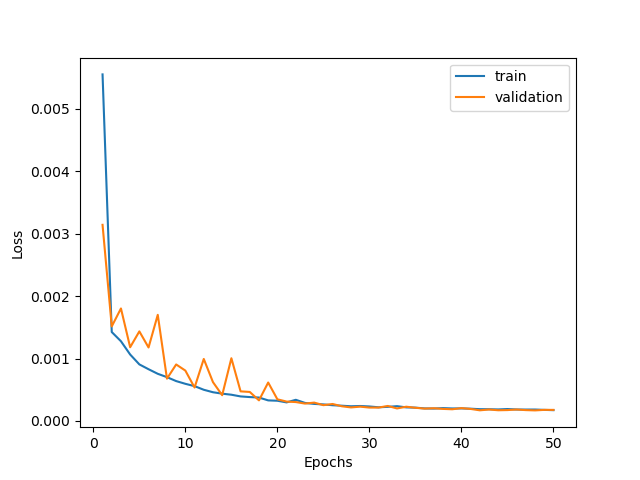
\includegraphics[width=0.8\linewidth]{../result/baseline_unet_data_aug.png}
  \caption{Training and Validation Loss for U-Net with Data Augmentation.}
  \label{fig:data_aug_loss}
\end{figure}

The baseline U-Net architecture trained with data augmentation on the training set resulted in the Dice coefficients shown in Table \ref{tab:data_aug_unet_comparison}.
\begin{table}[H]
  \centering
  \caption{Dice Coefficients: Baseline U-Net vs. U-Net with Data Augmentation (Task c)}
  \label{tab:data_aug_unet_comparison}
  \begin{tabular}{l|cc|cc}
    \toprule
    Structure & \multicolumn{2}{c|}{Baseline U-Net (DSC)} & \multicolumn{2}{c}{U-Net + Data Aug. (DSC)}                         \\
              & Mean Dice                                 & Std. Dev.                                   & Mean Dice & Std. Dev. \\
    \midrule
    RV        & 0.9519                                    & 0.0086                                      & 0.9276    & 0.0107    \\
    MYO       & 0.8734                                    & 0.0161                                      & 0.8469    & 0.0149    \\
    LV        & 0.8920                                    & 0.0310                                      & 0.8635    & 0.0384    \\
    \bottomrule
  \end{tabular}
\end{table}

\subsection{Discussion}
As shown in Table \ref{tab:data_aug_unet_comparison}, the specific data augmentation strategy employed led to a slight decrease in Dice coefficients for all structures compared to the baseline model trained on un-augmented data.
\begin{itemize}
  \item \textbf{DSC Decrease}: The specific augmentation strategy led to slightly lower Dice scores.
  \item \textbf{Possible Reasons}:
        \begin{itemize}
          \item Some aggressive augmentations (e.g., large rotations or shears in \texttt{RandomAffine}) could have distorted anatomical structures or altered their relative locations significantly, making it harder for the model to learn precise boundaries. Maybe the relative location of structures was altered too much.
        \end{itemize}
  \item \textbf{Conclusion}: While data augmentation is often beneficial, its effectiveness is highly dependent on the chosen transformations and the dataset. For this project, the selected augmentations did not improve performance and may have even been detrimental. The relative location of structures is crucial for segmentation tasks, and the specific augmentations used may not have been beneficial for this dataset. More careful selection, parameter tuning, or domain-specific augmentations would be necessary to potentially see benefits.
\end{itemize}


\section{U-Net with Soft Dice Loss}

\subsection{Structure}
\begin{itemize}
  \item \textbf{Network}: The baseline U-Net architecture (with skip connections) was used.
  \item \textbf{Training Data}: The original non-augmented training dataset was used for this experiment.
  \item \textbf{Loss Function Modification}: A \texttt{SoftDiceLoss} class was implemented. This loss calculates the Dice
        coefficient directly on the sigmoid probabilities of the model's output and the multi-channel binary ground truth. The
        loss is defined as $1 - \text{mean}(\text{Dice\_per\_class})$. A smoothing factor of 1.0 was added to the numerator and
        denominator to maintain stability.
  \item \textbf{Retraining}: The U-Net model was trained for 50 epochs using the \texttt{SoftDiceLoss}. The Adam optimizer was used with a learning rate of 0.001 and an ExponentialLR scheduler.
\end{itemize}

\subsection{Performance}
The training and validation loss curves for the U-Net trained with Soft Dice Loss are shown in Figure \ref{fig:soft_dice_loss_curve}.
\begin{figure}[H]
  \centering
  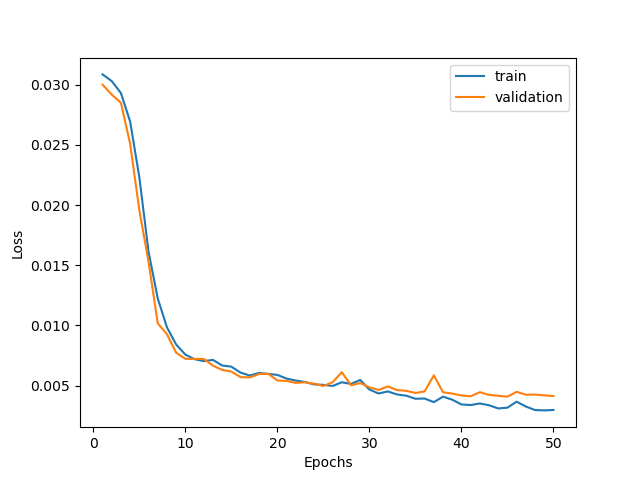
\includegraphics[width=0.8\linewidth]{../result/soft_dice_loss.png}
  \caption{Training and Validation Loss for U-Net with Soft Dice Loss.}
  \label{fig:soft_dice_loss_curve}
\end{figure}

The U-Net trained with Soft Dice Loss on the non-augmented dataset achieved the Dice coefficients shown in Table \ref{tab:soft_dice_unet_comparison} and pixel-wise accuracies in Table \ref{tab:soft_dice_unet_accuracy}.
\begin{table}[H]
  \centering
  \caption{Dice Coefficients: Baseline U-Net (BCE Loss) vs. U-Net (Soft Dice Loss) (Task d)}
  \label{tab:soft_dice_unet_comparison}
  \begin{tabular}{l|cc|cc}
    \toprule
    Structure & \multicolumn{2}{c|}{Baseline U-Net (BCE Loss)} & \multicolumn{2}{c}{U-Net (Soft Dice Loss)}                               \\
              & Mean Dice                                      & Std. Dev.                                  & Mean Dice       & Std. Dev. \\
    \midrule
    RV        & 0.9519                                         & 0.0086                                     & \textbf{0.9566} & 0.0100    \\
    MYO       & 0.8734                                         & 0.0161                                     & \textbf{0.8962} & 0.0100    \\
    LV        & 0.8920                                         & 0.0310                                     & \textbf{0.8998} & 0.0371    \\
    \bottomrule
  \end{tabular}
\end{table}

\begin{table}[H]
  \centering
  \caption{Pixel-wise Accuracy: Baseline U-Net (BCE Loss) vs. U-Net (Soft Dice Loss)}
  \label{tab:soft_dice_unet_accuracy}
  \begin{tabular}{l|cc|cc}
    \toprule
    Structure & \multicolumn{2}{c|}{Baseline U-Net (BCE Loss)} & \multicolumn{2}{c}{U-Net (Soft Dice Loss)}                               \\
              & Mean Accuracy                                  & Std. Dev.                                  & Mean Accuracy   & Std. Dev. \\
    \midrule
    RV        & 0.9991                                         & 0.0002                                     & \textbf{0.9992} & 0.0002    \\
    MYO       & 0.9977                                         & 0.0003                                     & \textbf{0.9980} & 0.0002    \\
    LV        & 0.9983                                         & 0.0005                                     & 0.9983          & 0.0006    \\
    \bottomrule
  \end{tabular}
\end{table}

Example segmentation results for the U-Net trained with Soft Dice Loss are shown in Figures \ref{fig:soft_dice_example_lv}, \ref{fig:soft_dice_example_myo}, and \ref{fig:soft_dice_example_rv}.
\begin{figure}[H]
  \centering
  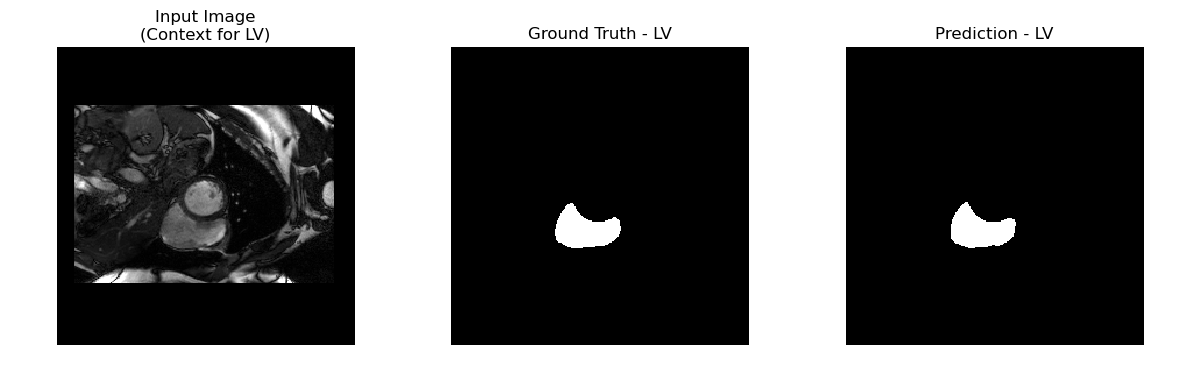
\includegraphics[width=\linewidth]{../result/for_ppt/soft_dice_loss_LV.png}
  \caption{U-Net with Soft Dice Loss Segmentation Example: LV}
  \label{fig:soft_dice_example_lv}
\end{figure}
\begin{figure}[H]
  \centering
  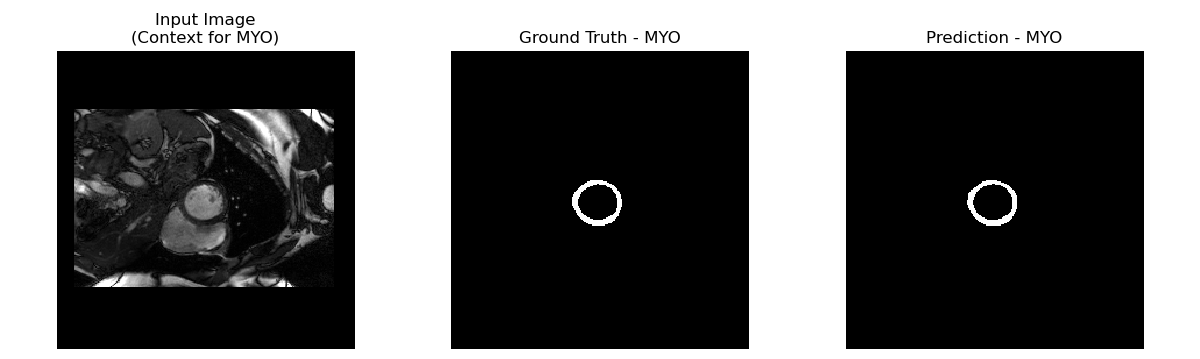
\includegraphics[width=\linewidth]{../result/for_ppt/soft_dice_loss_MYO.png}
  \caption{U-Net with Soft Dice Loss Segmentation Example: MYO}
  \label{fig:soft_dice_example_myo}
\end{figure}
\begin{figure}[H]
  \centering
  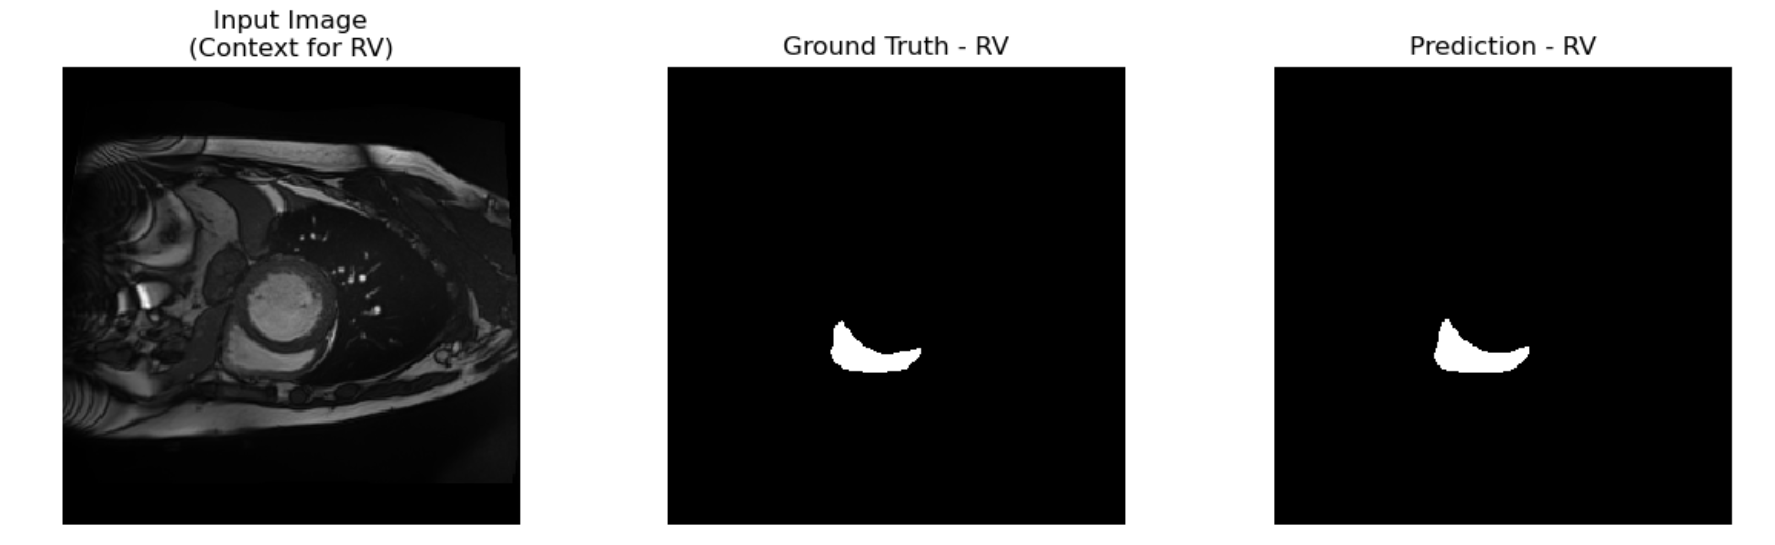
\includegraphics[width=\linewidth]{../result/for_ppt/soft_dice_loss_RV.png}
  \caption{U-Net with Soft Dice Loss Segmentation Example: RV}
  \label{fig:soft_dice_example_rv}
\end{figure}

\subsection{Discussion}
As shown in Table \ref{tab:soft_dice_unet_comparison} and Table \ref{tab:soft_dice_unet_accuracy}:
\begin{itemize}
  \item \textbf{Segmentation Accuracy (Dice)}: Using Soft Dice Loss resulted in noticeably better Dice coefficients for all cardiac structures compared to BCE Loss when trained on the same non-augmented data. The improvement for MYO was particularly significant (0.8734 to 0.8962).
  \item \textbf{Segmentation Accuracy (Pixel-wise)}: Pixel-wise accuracy also showed slight improvements or remained comparable at very high levels.
  \item \textbf{Conclusion for Task (d)}: Changing the training loss from cross-entropy (BCE) to Soft Dice Loss improved overall segmentation accuracy, especially when evaluated by the Dice coefficient, which is more sensitive to segmentation overlap and robust to class imbalance.
\end{itemize}


\section{Improvements}
To further enhance segmentation performance, an Attention U-Net architecture and a Hybrid Loss function were implemented and evaluated.

\subsection{Attention U-Net}
\subsubsection{Structure}
\begin{itemize}
  \item \textbf{Advanced U-Net (Attention U-Net):}
        \begin{itemize}
          \item \textbf{Architecture:} An \texttt{AttentionBlock} was introduced in the decoder's \texttt{Up} module. The \texttt{AttentionBlock} computes attention coefficients by combining features from the decoder (gating signal) and the corresponding skip connection from the encoder. These coefficients are then applied to the encoder features, effectively allowing the model to focus on more relevant spatial regions during the upsampling and feature fusion process. This helps in refining segmentation boundaries, especially for complex structures. The architecture is depicted in Figure \ref{fig:attention_unet_architecture}.
        \end{itemize}
  \item \textbf{Loss Function:} \texttt{SoftDiceLoss} was used, given its superior performance in the previous experiment.
  \item \textbf{Optimizer:} Adam optimizer with a learning rate of 0.001 and an ExponentialLR scheduler.
  \item \textbf{Training:} The model was trained for 50 epochs on the non-augmented training dataset.
\end{itemize}

\begin{figure}[H]
  \centering
  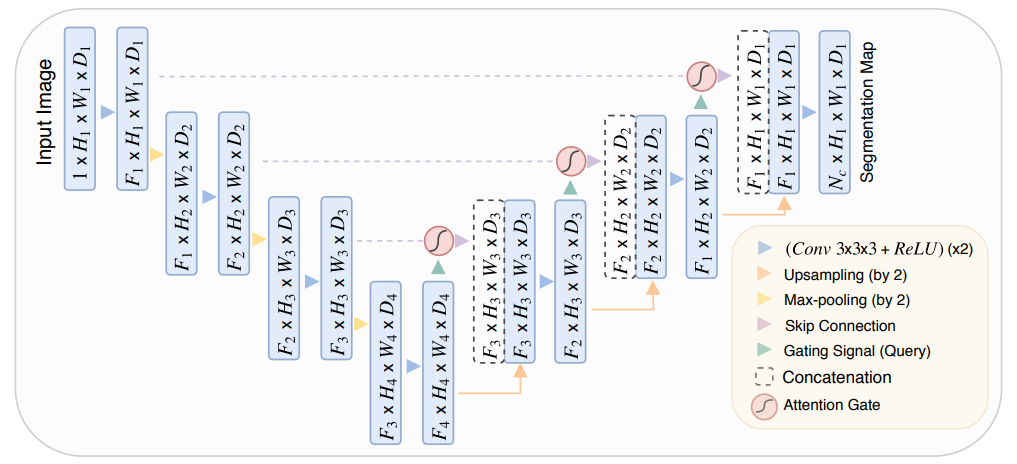
\includegraphics[width=\linewidth]{../result/for_ppt/attention_unet.png}
  \caption{Attention U-Net Architecture.}
  \label{fig:attention_unet_architecture}
\end{figure}

\subsubsection{Performance}
The Attention U-Net trained with Soft Dice Loss achieved the Dice coefficients shown in Table \ref{tab:attention_unet_comparison}.
\begin{table}[H]
  \centering
  \caption{Dice Coefficients: Baseline (BCE), Baseline (Soft Dice Loss), and Attention U-Net (Soft Dice Loss) (Task e.1)}
  \label{tab:attention_unet_comparison}
  \begin{tabular}{l|cc|cc|cc}
    \toprule
    Structure & \multicolumn{2}{c|}{Baseline U-Net (BCE)} & \multicolumn{2}{c|}{U-Net (Soft Dice)} & \multicolumn{2}{c}{Attention U-Net (Soft Dice)}                                           \\
              & Mean Dice                                 & Std. Dev.                              & Mean Dice                                       & Std. Dev. & Mean Dice       & Std. Dev. \\
    \midrule
    RV        & 0.9519                                    & 0.0086                                 & 0.9566                                          & 0.0100    & \textbf{0.9588} & 0.0086    \\
    MYO       & 0.8734                                    & 0.0161                                 & 0.8962                                          & 0.0100    & \textbf{0.8967} & 0.0109    \\
    LV        & 0.8920                                    & 0.0310                                 & \textbf{0.8998}                                 & 0.0371    & 0.8972          & 0.0492    \\
    \bottomrule
  \end{tabular}
\end{table}

Example segmentation results for the Attention U-Net are shown in Figures \ref{fig:attention_unet_example_lv}, \ref{fig:attention_unet_example_myo}, and \ref{fig:attention_unet_example_rv}.
\begin{figure}[H]
  \centering
  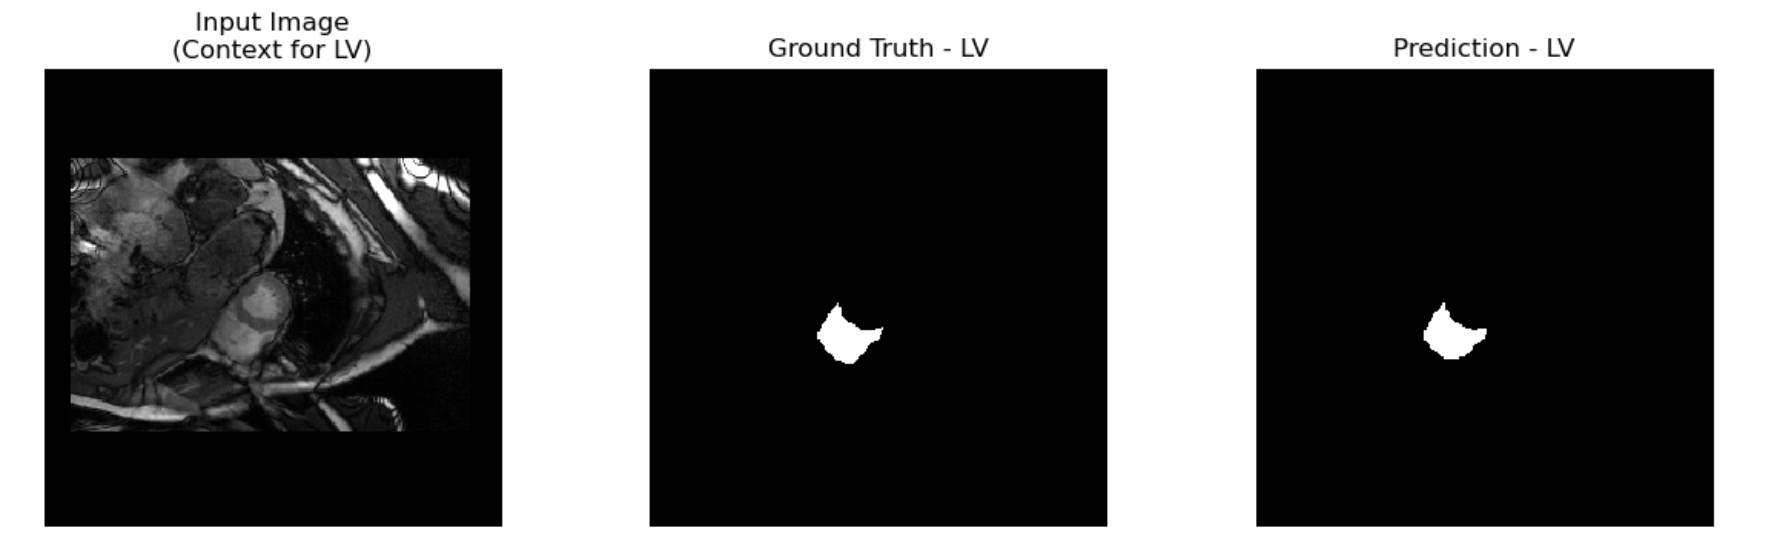
\includegraphics[width=\linewidth]{../result/for_ppt/attention_LV.png}
  \caption{Attention U-Net Segmentation Example: LV}
  \label{fig:attention_unet_example_lv}
\end{figure}
\begin{figure}[H]
  \centering
  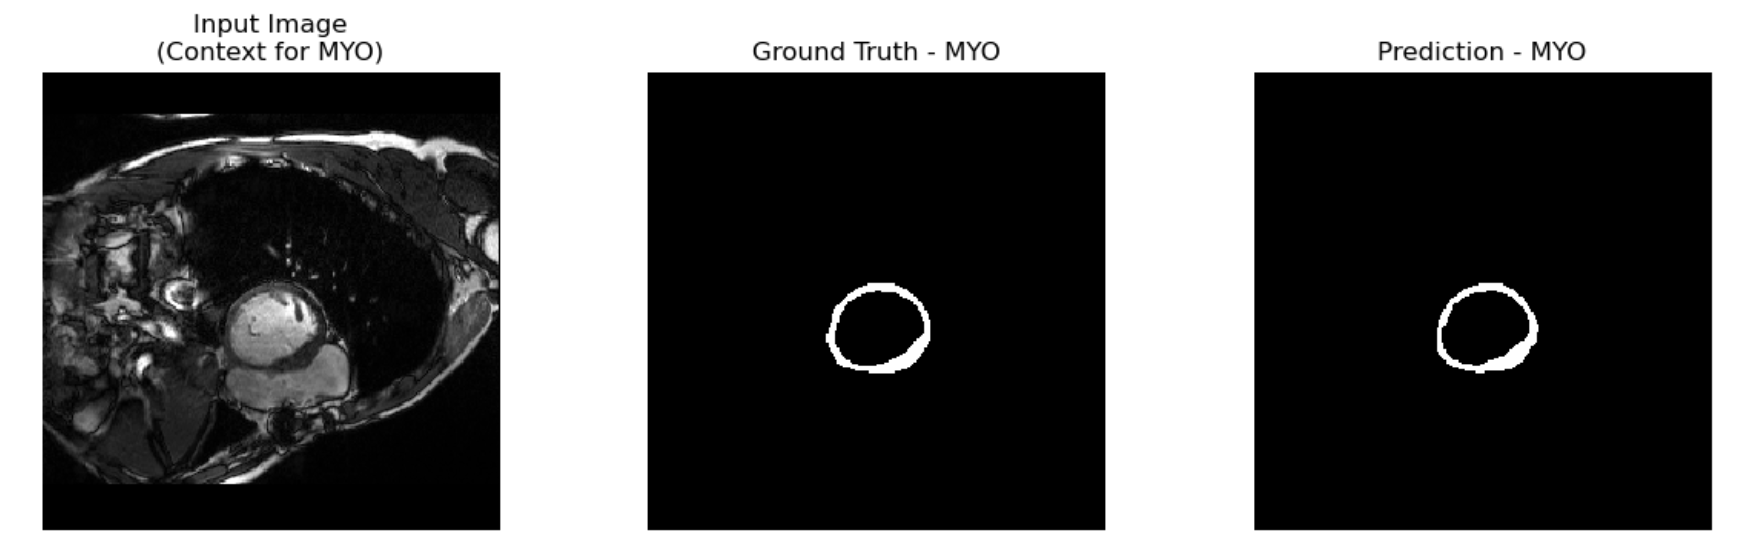
\includegraphics[width=\linewidth]{../result/for_ppt/attention_MYO.png}
  \caption{Attention U-Net Segmentation Example: MYO}
  \label{fig:attention_unet_example_myo}
\end{figure}
\begin{figure}[H]
  \centering
  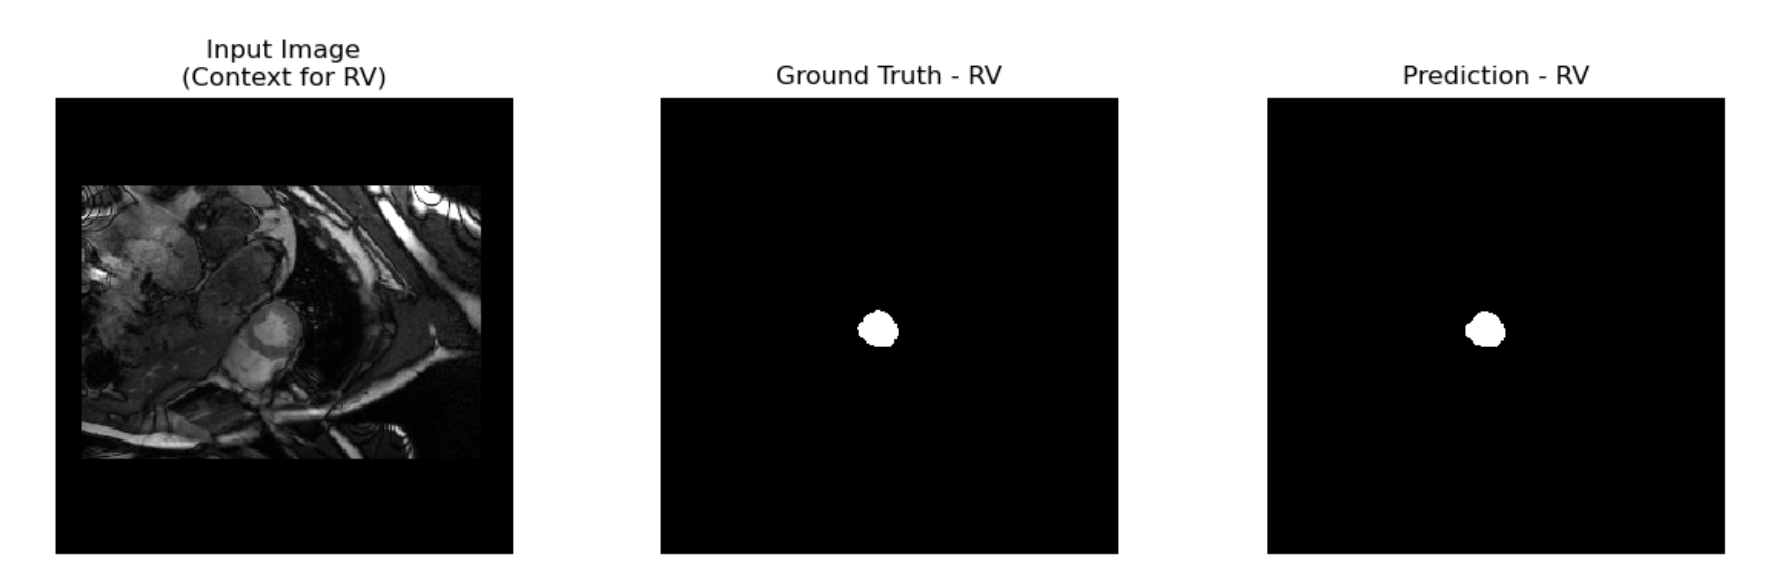
\includegraphics[width=\linewidth]{../result/for_ppt/attention_RV.png}
  \caption{Attention U-Net Segmentation Example: RV}
  \label{fig:attention_unet_example_rv}
\end{figure}

\subsubsection{Discussion}
\begin{itemize}
  \item The Attention U-Net showed improved Dice scores for RV and MYO compared to the baseline U-Net with BCE loss and the U-Net with Soft Dice Loss. For LV, the performance was comparable to the U-Net with Soft Dice Loss.
  \item This suggests that the attention mechanism effectively helps the model to focus on more complex structures or finer details, leading to better boundary delineation for RV and MYO.
  \item Accuracy scores (not shown in table, but generally high) are very high across all structures, which is common in segmentation tasks with large background areas. The Dice coefficient remains a more informative metric for evaluating overlap.
\end{itemize}

\subsection{Hybrid Loss}
\subsubsection{Motivation}
To further improve segmentation, especially at boundaries and for complex structures, by combining multiple complementary loss objectives. This aims to leverage the strengths of different loss types for a more holistic optimization.

\subsubsection{HybridLoss Structure}
The HybridLoss adaptively weights four distinct loss components:
\begin{enumerate}
  \item \textbf{Dice Loss} (Overlap)
  \item \textbf{Binary Cross-Entropy (BCE) Loss} (Pixel-wise accuracy)
  \item \textbf{Boundary Loss} (Edge definition)
  \item \textbf{Hausdorff Distance Loss (Approximation)} (Shape similarity)
\end{enumerate}
The implementation features adaptive weighting of these components using learnable uncertainty parameters. Both the standard U-Net and Attention U-Net were trained with this HybridLoss on non-augmented data.

\subsubsection{Performance with HybridLoss}
The mean Dice scores for models trained with HybridLoss are presented in Table \ref{tab:hybridloss_results}.
\begin{table}[H]
  \centering
  \caption{Mean Dice Scores with HybridLoss (Task e.2, e.3)}
  \label{tab:hybridloss_results}
  \begin{tabular}{l|c|c|c}
    \toprule
    Model Configuration                  & RV Dice (SD)             & MYO Dice (SD)            & LV Dice (SD)             \\
    \midrule
    U-Net + HybridLoss                   & 0.9504 (0.0276)          & 0.8839 (0.0275)          & \textbf{0.9061} (0.0573) \\
    \textit{Baseline U-Net (BCE)}        & \textit{0.9519 (0.0086)} & \textit{0.8734 (0.0161)} & \textit{0.8920 (0.0310)} \\
    \midrule
    Attention U-Net + HybridLoss         & 0.9507 (0.0235)          & 0.8875 (0.0247)          & 0.9033 (0.0703)          \\
    \textit{Attention U-Net (Soft Dice)} & \textit{0.9588 (0.0086)} & \textit{0.8967 (0.0109)} & \textit{0.8972 (0.0492)} \\
    \bottomrule
  \end{tabular}
\end{table}


\section{Overall Performance Summary}
Table \ref{tab:overall_summary} provides a consolidated view of the mean Dice Similarity Coefficients (DSC) for all evaluated models across the three cardiac structures.

\begin{table}[H]
  \centering
  \caption{Overall Performance Summary: Mean Dice Coefficients}
  \label{tab:overall_summary}
  \begin{tabular}{lccc}
    \toprule
    Model Configuration                             & RV Mean DSC     & MYO Mean DSC    & LV Mean DSC     \\
    \midrule
    (a) Baseline U-Net (BCE Loss)                   & 0.9519          & 0.8734          & 0.8920          \\
    (b) U-Net without Skip Connections (BCE Loss)   & 0.9260          & 0.8223          & 0.8588          \\
    (c) U-Net + Data Augmentation (BCE Loss)        & 0.9276          & 0.8469          & 0.8635          \\
    (d) U-Net (Soft Dice Loss, No Aug.)             & 0.9566          & 0.8962          & 0.8998          \\
    (e.1) Attention U-Net (Soft Dice Loss, No Aug.) & \textbf{0.9588} & \textbf{0.8967} & 0.8972          \\
    (e.2) U-Net + HybridLoss (No Aug.)              & 0.9504          & 0.8839          & \textbf{0.9061} \\
    (e.3) Attention U-Net + HybridLoss (No Aug.)    & 0.9507          & 0.8875          & 0.9033          \\
    \bottomrule
  \end{tabular}
\end{table}

\section{Overall Discussion}
The results from Table \ref{tab:overall_summary} highlight several key observations:
\begin{itemize}
  \item The Attention U-Net with Soft Dice Loss (e.1) achieved the best performance for RV and MYO segmentation.
  \item The standard U-Net combined with HybridLoss (e.2) yielded the highest Dice score for LV segmentation.
  \item No Universal Superiority of HybridLoss: Despite its sophisticated multi-component design with adaptive weighting, HybridLoss did not prove to be a universally superior loss function across all structures and base architectures in these experiments. For RV and MYO, the simpler Soft Dice Loss with Attention U-Net performed better.
  \item LV Segmentation Strength with HybridLoss: A consistent observation is the relative strength of HybridLoss (or its components) in improving or maintaining high performance for LV segmentation, even when RV/MYO performance might not be optimal compared to other configurations. This suggests that the combined objectives in HybridLoss might be particularly beneficial for the characteristics of the LV.
\end{itemize}


\section{Conclusion}
This project successfully implemented and evaluated several U-Net based models for cardiac cine MRI segmentation. Key findings include:
\begin{enumerate}
  \item The baseline U-Net provides a strong starting point for segmenting RV, LV, and MYO.
  \item Skip connections are essential for U-Net's performance. Their removal led to a significant decline in Dice scores.
  \item The specific data augmentation strategy employed resulted in a decrease in Dice coefficients, highlighting that augmentation strategies must be carefully chosen and tuned.
  \item Training with Soft Dice Loss significantly improved performance over Binary Cross-Entropy loss, particularly for the more challenging MYO structure.
  \item The Attention U-Net with Soft Dice Loss yielded the best segmentation performance for RV (0.9588 DSC) and MYO (0.8967 DSC).
  \item The U-Net with HybridLoss achieved the best result for LV segmentation (0.9061 DSC).
  \item The choice of loss function and architectural enhancements like attention mechanisms can lead to notable improvements, but their effectiveness can be structure-dependent. A simpler model (U-Net) with a well-chosen, targeted loss function (Soft Dice Loss) can still be highly effective.
  \item The performance of HybridLoss models suggests that further optimization (e.g., training duration, hyperparameter tuning of the loss components or solver) could potentially lead to even better results.
\end{enumerate}
Future work could explore more sophisticated data augmentation techniques, further investigate different loss function combinations, or experiment with different attention mechanisms or network backbones.


\end{document}